
%%%%%%%%%%%%%%%%%%%%%%% file typeinst.tex %%%%%%%%%%%%%%%%%%%%%%%%%
%
% This is the LaTeX source for the TDPTemplate using
% the LaTeX document class 'llncs.cls' Springer LNAI format
% used in the RoboCup Symposium submissions.
% http://www.springer.com/computer/lncs?SGWID=0-164-6-793341-0
%
% It may be used as a template for your own TDP - copy it
% to a new file with a new name and use it as the basis
% for your Team Description Paper
%
% NB: the document class 'llncs' has its own and detailed documentation, see
% ftp://ftp.springer.de/data/pubftp/pub/tex/latex/llncs/latex2e/llncsdoc.pdf
%
%%%%%%%%%%%%%%%%%%%%%%%%%%%%%%%%%%%%%%%%%%%%%%%%%%%%%%%%%%%%%%%%%%%

\documentclass[runningheads,a4paper]{llncs}
\usepackage{amssymb}
\setcounter{tocdepth}{3}
\usepackage{graphicx}
\usepackage{amssymb}
\usepackage[utf8]{inputenc}
\usepackage{url}
\usepackage{float}
\usepackage{amsmath}
\usepackage{graphicx}
\usepackage{wrapfig}
\usepackage{tabto}
\usepackage{lipsum}
\usepackage[table,xcdraw]{xcolor}
\usepackage{hyperref}
\usepackage{subcaption}
\usepackage[T1]{fontenc}

\newcommand\notes[1]{\textcolor{red}{#1}}


\begin{document}


\newif\ifdraft
\draftfalse


\ifdraft
\setlength{\belowcaptionskip}{-5pt}
\fi

\title{Walking Machine @Home \newline \: 2019 Team Description Paper}

\author{Jeffrey Cousineau, Huynh-Anh Le, et al.}
\institute{École de Technologie Supérieure \\ 1100 rue Notre-Dame Ouest, Montreal, QC, Canada H3C 1K3 \\
\texttt{http://walkingmachine.ca,} \texttt{walking@ens.etsmtl.ca,} \texttt{https://github.com/WalkingMachine}}
\maketitle


%%%%%%%%%%%%%%%%%%%%%%%%%%%%%%%%%%%%%%%%%%%%%%%%%%%%%%%%%%%%%%%%%%%%%%%%%%%%%%%%%%%%

\begin{abstract}

This paper gives details about the RoboCup@Home league team Walking Machine, from ETS University in Montreal, Canada for the next competition in Sydney, Australia in July 2019. The robot from Walking Machine named, S.A.R.A. for "Systeme d'Assistance Robotique Autonome" (in English, Automated Robotic Assistance System), is a robot entirely built by the scientific club from ETS, mainly composed of undergraduates students. The robot is used for social interaction with humans, navigation and object manipulation. This document shows the electrical, mechanical and software novelties and functionalities of S.A.R.A.

\end{abstract}

%%%%%%%%%%%%%%%%%%%%%%%%%%%%%%%%%%%%%%%%%%%%%%%%%%%%%%%%%%%%%%%%%%%%%%%%%%%%%%%%%%%%

\section{Introduction}
\tab Walking Machine’s team is a young team from Montreal, Quebec, in Canada, composed of engineering students in the field of mechanical, electrical and software engineering. We have been working really hard to improve our robot for next year's RoboCup@Home competition. As this would be our fourth participation, we learned a lot at RoboCup Montreal and we made many improvements to get better results, mostly on the software side. In the past, the team went in many competitions like the Eurobot but made the leap for the RoboCup@Home competition to get a bigger challenge and to get an opportunity to bring novelty in the scientific community surrounding robotics.\\

S.A.R.A. was designed for polyvalent human-robot interaction as well as efficient navigation and object manipulation. Our robot is mounted on four mecanum wheels, have a 7 DoF arm and use sensors for communication and navigation. Our team has developed knowledge in the object and people detection/recognition, as well as navigation using a laser scanner and an Asus Xtion camera. All of these parts are interfaced through ROS(Robot Operating System). \\

In the rest of this paper, we will present in the mechanical improvements we've made to our robot to overcome the different challenge, the different packages we've developed are described, and finally, this paper will conclude and explore the expected features for next year Robocup.


\section{Mechanical improvement}

\tab To improve our robot abilities, we decided to add a vertical linear actuator, more specifically, a TL5 column made by TiMOTION. This will add a degree of freedom, giving us a wider range of motion to reach objects on the floor or higher on the cupboard shelves. This will be really helpful for a challenge like storing groceries where the objects can be anywhere in the cupboard. \\

\begin{figure}[h!]
  \centering
  \begin{subfigure}[b]{0.15\linewidth}
    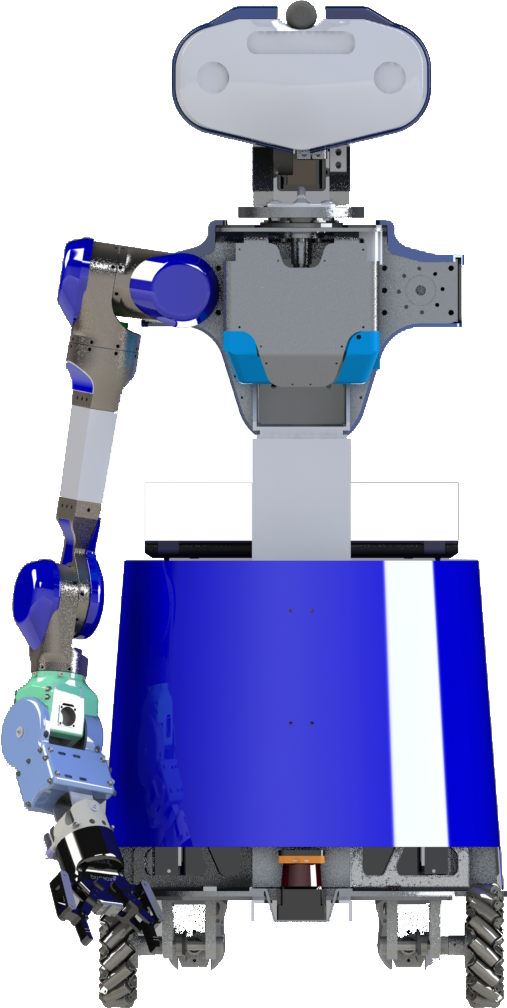
\includegraphics[width=\linewidth]{images/sara_render_retracted.png}
    \caption{Robot retracted}
  \end{subfigure}
  \hspace{1.5cm}
  \begin{subfigure}[b]{0.15\linewidth}
    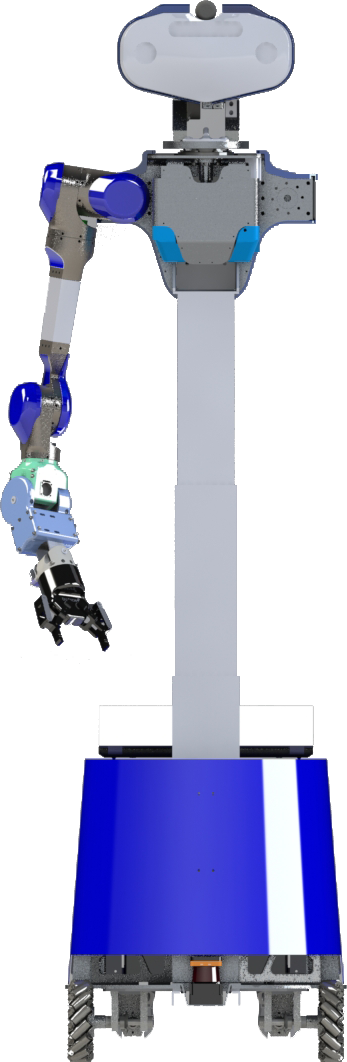
\includegraphics[width=\linewidth]{images/sara_render_extracted.png}
    \caption{Robot extracted}
  \end{subfigure}
  \caption{S.A.R.A. linear actuator motion range}
  \label{fig:coffee}
\end{figure}

We also decided to improve our wrist by adding a gearbox, giving it more strength. We took the decision to improve it after having problems with the gripper being too heavy. 

\begin{figure}
  \centering
  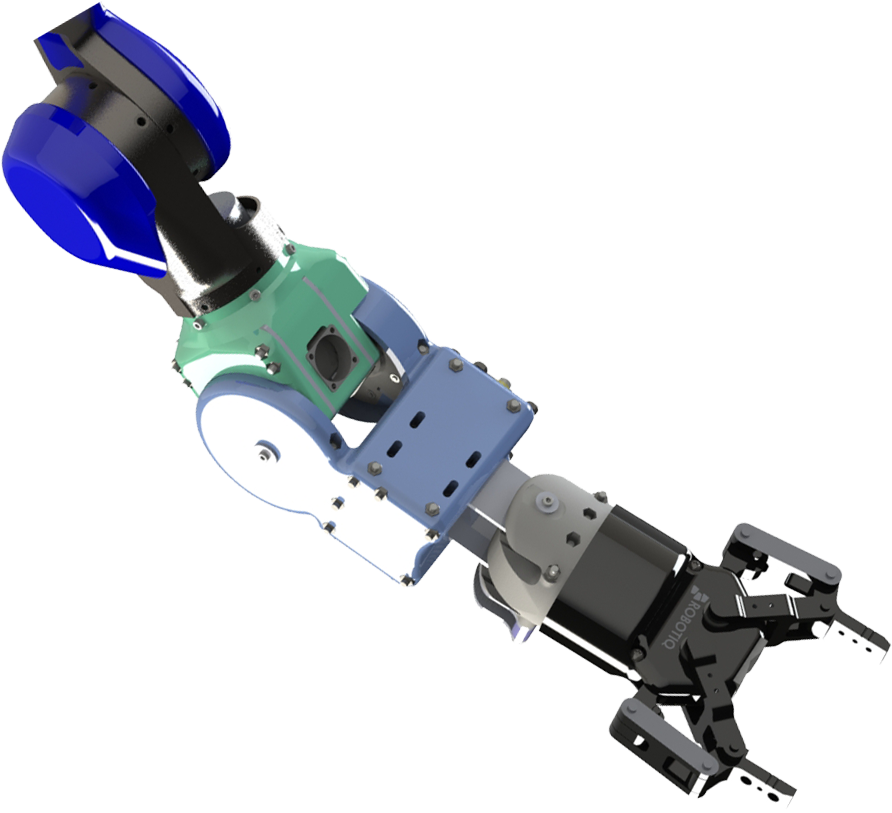
\includegraphics[width=125pt]{images/wrist.png}
  \caption{Improved wrist 3D render}
\end{figure} 

\newpage
\section{Software}

\subsection{Natural language understanding}

\tab To convert spoken data in actions subset, we had to create our own natural language understanding system (\href{http://github.com/walkingmachine/wm\_nlu}{http://github.com/walkingmachine/wm\_nlu}). To pursue our goal, we based ourself on rasa nlu\cite{rasa}, an open-source NLP tool for intent classification and entity extraction. Altough, a simple entity extraction wasn't enough for us, we wanted a system that would take a command as an input and output the desired actions.\\

To make this work, our first step was to create a dataset for the entity classification. Based on the GPSRCmdGen, we generated sentences which we hand labeled by attributing an entity to each specific type of sentence paired with specific parameters.\\

We then built a ROS service which takes a sentence as an input, classify the main intent using our dataset and return an array of actions that the robot needs to execute according to the command. Our system is dependent on our environment representation package(\href{http://github.com/walkingmachine/wonderland}{http://github.com/walkingmachine/wonderland}) since queries are made to our database.

\begin{figure}
  \centering
  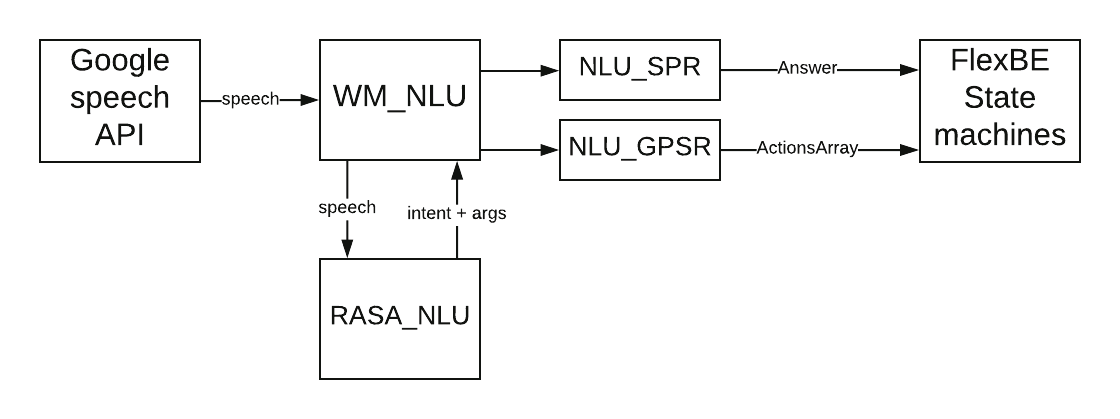
\includegraphics[width=300pt]{images/wm_nlu.png}
  \caption{Natural language understanding process}
\end{figure} 

\subsection{Sound localization}
\tab To improve our performances mainly in the SPR challenge and to add reactivity to our robot, we decided to add a Matrix Creator which includes a microphone array coupled with a Raspberry Pi 3. We decided to use ODAS  \cite{odas} which stands for Open embeddeD Audition System. This is a library dedicated to performing sound source localization, tracking, separation and post-filtering, developed by IntRoLab\cite{Introlab} from Sherbrooke University in Quebec.\\ 

\begin{figure}
  \centering
  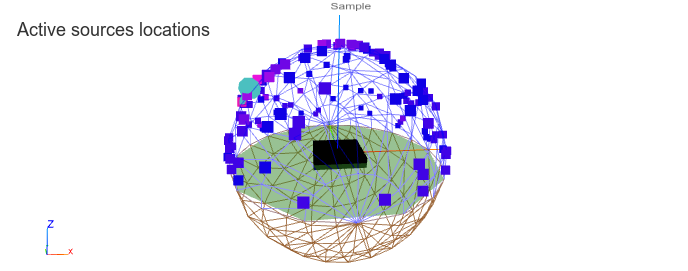
\includegraphics[width=300pt]{images/odas.png}
  \caption{ sound source localization from ODAS web visualizer \cite{odas}}
\end{figure} 

At first, a simple sound source localization is used. Then a Kalman filter is applied to perform sound source tracking. It helps us eliminate simple noise to track the person talking to the robot. We can even go further with this library by using the sound source separation which helps us separate the sound incoming from the different audio sources.\\

We decided to build our own ROS wrapper around ODAS considering the lack of documentation surrounding the project. Our wrapper offers multiple topics which publish either the different sound sources location, the tracked sound sources or the separated sound sources. We can then easily identify the location of an operator giving a command to our robot.\\

\subsection{Object recognition}
\subsubsection{Recognition system}
\hfill\\

For our object recognition, we use YOLO \cite{yolo}, a real-time object detection. It does not only detect various object but it also predicts the bounding boxes of the detected object. It uses a single neural network which is applied to the image. Multiple regions are then created and are used to predict the bounding boxes. Each of them also contains the predicted probability which is used to filter the predicted objects. The advantages of this system is that it can detect multiple objects in a real-time scenario.\\

\begin{figure}[h!]
  \centering
  \begin{subfigure}[b]{0.43\linewidth}
    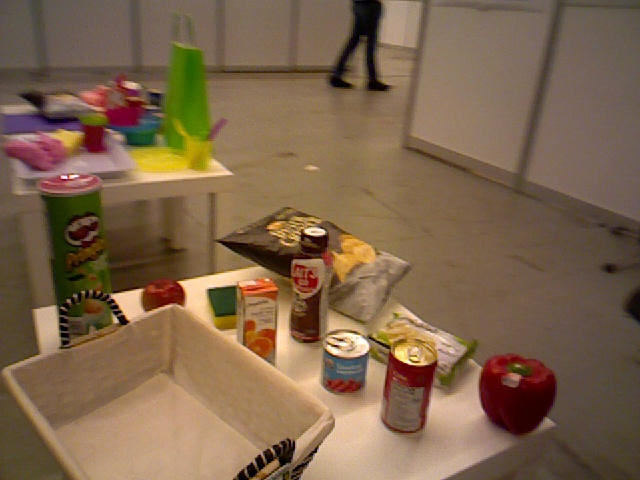
\includegraphics[width=\linewidth]{images/input_objects.JPEG}
    \caption{Input image}
  \end{subfigure}
  \hspace{1.5cm}
  \begin{subfigure}[b]{0.43\linewidth}
    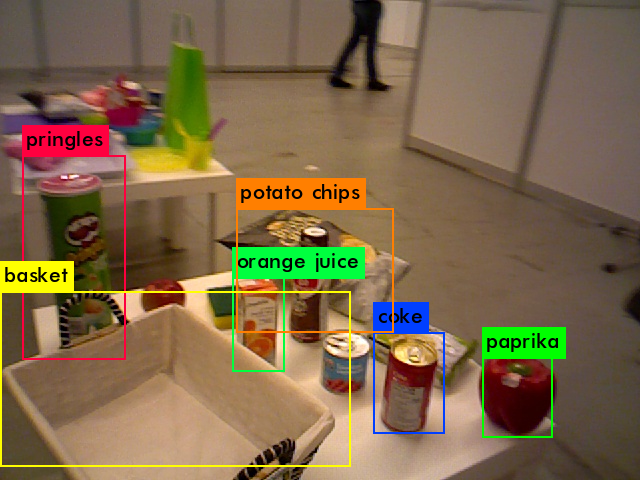
\includegraphics[width=\linewidth]{images/output_objects.png}
    \caption{Output image}
  \end{subfigure}
  \caption{Custom model trained during Robocup 2018}
  \label{fig:coffee}
\end{figure} 

\subsubsection{Dataset creation tool}
\hfill\\

This year we are putting our efforts on a way to simplify the dataset creation. During the last RoboCup in Montreal, it was the first time our team had an efficient object recognition system. However, our flaw was in the production of our dataset. Since we are retraining over ImageNet's pre-trained weight, we need to provide a large dataset and for this, we had to do all the bounding boxes by hand for every images.\\
 
We decided that we needed to find a faster way to train the provided objects from the arena. Our plan is now to use a rotating platform with a green screen, that way we could automate the data collection process by using background subtraction technique with OpenCV and contour detection to find the object bounding box. Using the subtracted object, we can now apply different transformations to do dataset augmentation. \\

For the moment, we only created the software part to automated the bounding boxes. As you can see, on the Fig.6 a), we applied an inRange filter, on the Fig.6 b), we inverted the image to finally apply the findContour function on Fig.6 c). By taking the largest contour found, we can easily calculate the bounding box of the object.  \\
 
\begin{figure}[h!]
  \centering
  \begin{subfigure}[b]{0.3\linewidth}
    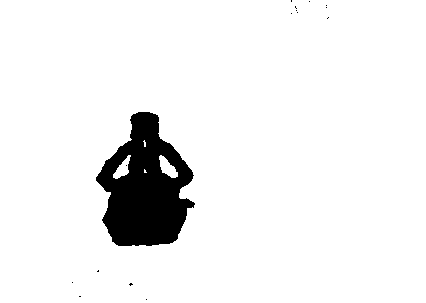
\includegraphics[width=\linewidth]{images/bounding_inrange.png}
    \caption{InRange filter}
  \end{subfigure}
  \begin{subfigure}[b]{0.3\linewidth}
    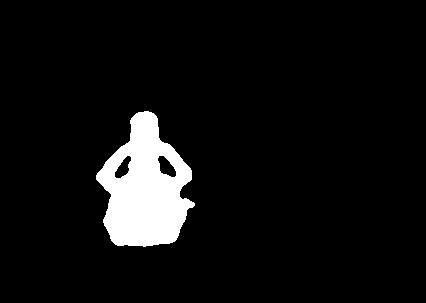
\includegraphics[width=\linewidth]{images/bounding_invert.png}
    \caption{Invert image}
  \end{subfigure}
  \begin{subfigure}[b]{0.3\linewidth}
    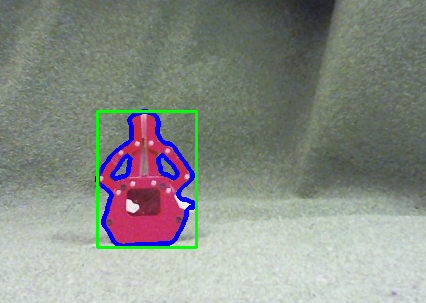
\includegraphics[width=\linewidth]{images/bounding_contours.png}
    \caption{Contour detection}
  \end{subfigure}
  \caption{Dataset creation process with wm\_dataset\_preparation}
  \label{fig:coffee}
\end{figure}  
 
\subsection{Environment modeling}
\tab To have a good representation of the robot's environment, we developed our own environment modeling called Wonderland. For this, we can insert in our database all the known information like the furniture, the rooms, and the objects. Based on this, our robot will interact with the database through a web API, which makes it ROS agnostic and could be used by any application even if it's not robotics oriented.\\

\begin{figure}
  \centering
  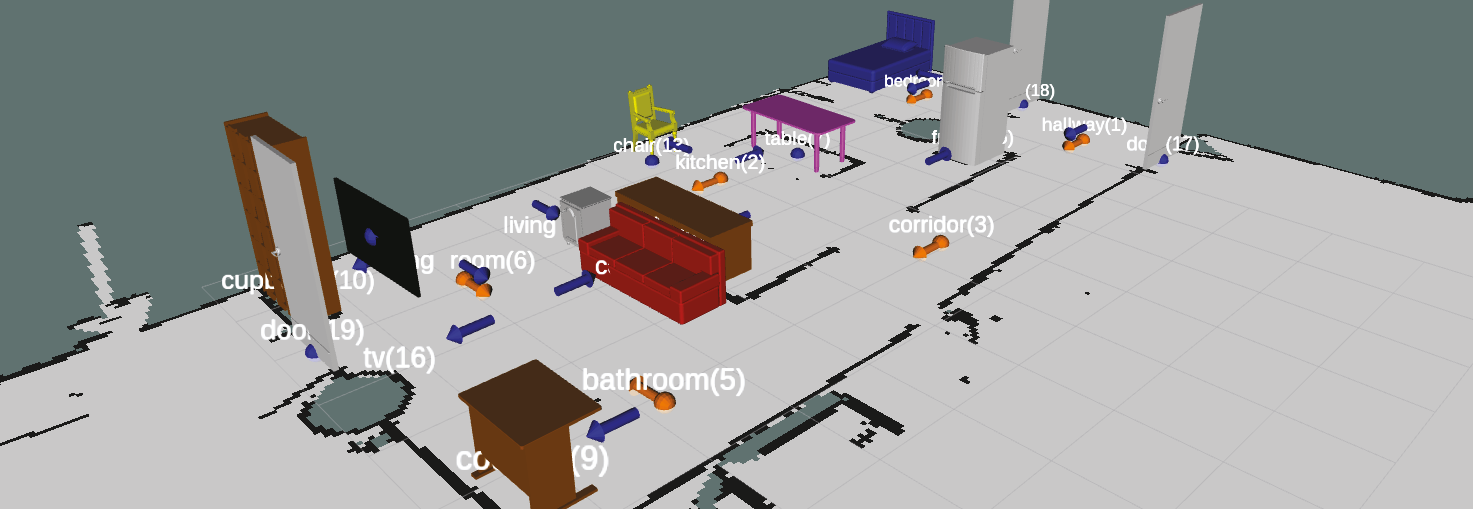
\includegraphics[width=300pt]{images/wonderland.png}
  \caption{ wm\_data\_collector process}
\end{figure} 

To make our life easier, we also implemented an easy way to place the object's position through Rviz. For the moment, we use the pose estimation tool however we are planning to develop our own tool in Rviz next year.\\

With our environment modeling system, our NLU node can interact with it to confirm that a query is valid by verifying, for example, the existence of a specific room or a specific object.  \\

\section{Objects and people tracking}

\tab To keep track of the many objects and people our robot sees, we have developed our tracking system named wm\_data\_collector \cite{datacollector}. Our process, as you can see on Fig8, imply the use of our various sensors to keep track of different characteristics defining our tracked entities. Once we gather the information, we use a simple Kalman filter but we are planning to use a better algorithm in the future like dlib correlation tracker. \\

\begin{figure}
  \centering
  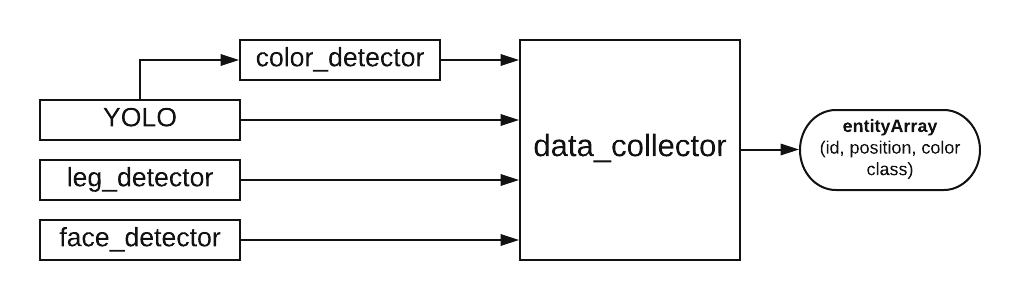
\includegraphics[width=300pt]{images/wm_data_collector.png}
  \caption{ wm\_data\_collector process}
\end{figure} 


\section{Conclusions and future work} 
\tab In this paper, we presented how we are developing our own robotic platform for the RoboCup@Home competition. It has many abilities like a person and gender recognition, pose detection, environmental reasoning, object recognition, manipulation and many more. Since we are mainly undergraduate students with no teacher support, our main efforts go in the learning process and the implementation part. Despite a low scientific contribution, we are actually developing some package that we hope will be usable by other teams in a near future.\\

This year we are planning to implement gesture recognition for the restaurant challenge and, planar and object segmentation to detect unknown objects mainly for the storing groceries challenge. For this, we'll simply use PCL library with the RANSAC algorithm using a plane model and the K-mean algorithm for object segmentation. Finally, we'll also be working to improve our Natural Language Understanding package to add more features for the more complex challenges in the GPSR.\\ 

\nocite{*}
\bibliographystyle{plain}
\bibliography{references}

\section*{Robot SARA Hardware Description}
% TODO Change picture and description
Specifications for robot SARA are as follows:

\begin{table}

\label{my-label}

\begin{tabular}{l|p{90mm}}
\hline
\rowcolor[HTML]{FFFFFF} 
\multicolumn{2}{c}{\cellcolor[HTML]{FFFFFF}\textbf{SARA}}                                                      \\ \hline
\rowcolor[HTML]{EAEFF6} 
\textbf{Base}               & Custom base with fully holonomic platform                                        \\
\rowcolor[HTML]{FFFFFF} 
\textbf{Right arm}          & 7 DoF custom arm made of Kinova motors                                           \\
\rowcolor[HTML]{EAEFF6} 
\textbf{Neck}               & Tilt and pan unit using two Dynamixel MX-64R servo actuator                      \\
\rowcolor[HTML]{FFFFFF} 
\textbf{Head}               & Custom head made of RGB neopixels leds and Asus Xtion Pro                        \\
\rowcolor[HTML]{EAEFF6} 
\textbf{Gripper}            & Robotiq 2 fingers 140mm                                                           \\
\rowcolor[HTML]{FFFFFF}
\textbf{Dimensions}         & \begin{tabular}[c]{@{}l@{}}Base : 0,61m. X 0,77m.\\ Height : 1,68m.\end{tabular} \\
\rowcolor[HTML]{EAEFF6} 
\textbf{Weight}             & $\sim$60kg                                                                      \\
\rowcolor[HTML]{FFFFFF} 
\textbf{Additional sensors} & Hokuyo UTM-30LX on base                                                          \\
\rowcolor[HTML]{EAEFF6} 
\textbf{Microphone}         & Rode microphone											                         \\
\rowcolor[HTML]{FFFFFF} 
\textbf{Batteries}          & 2x 20V Dewalt drill battery 5aH                                                 \\
\rowcolor[HTML]{EAEFF6} 
\textbf{Computer}           & 1x Lenovo p50 with 32GB RAM and nVidia Quadro M2000 4GB, 1x Raspberry Pi 3       \\ \hline
\end{tabular}
\caption{Robot's hardware description}
\end{table}
\begin{wrapfigure}[10]{r}{0.25\textwidth}
	\centering
	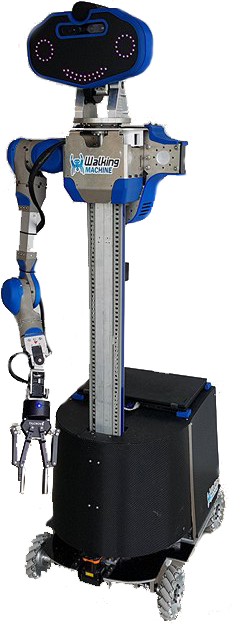
\includegraphics[width=0.30\textwidth]{images/sara_2.png}
	\caption{Robot SARA}
\end{wrapfigure}
\section*{Robot's Software Description}

For our robot we are using the following software:

\begin{itemize}
	\item Platform: Robotic Operating System (ROS) Kinetic on Ubuntu 16.04
	\item Navigation, localization and mapping: \href{http://wiki.ros.org/gmapping}{Gmapping}, \href{http://wiki.ros.org/amcl}{AMCL}, \href{http://wiki.ros.org/pointcloud_to_laserscan}{pointcloud\_to\_laserscan}
	\item Face recognition: \href{http://wiki.ros.org/people}{People}
	\item Speech recognition: \href{https://github.com/WalkingMachine/lab_ros_speech_to_text}{Google Speech API}
	\item Speech comprehension: \href{http://sag.art.uniroma2.it/lu4r.html}{LU4R}, \href{https://github.com/WalkingMachine/lu4r_ros}{lu4r\_ros}
	\item Speech generation: \href{https://doc.ubuntu-fr.org/svoxpico}{Svoxpico}
	\item Object recognition: \href{https://github.com/WalkingMachine/wm_darknet}{Darknet with YOLO v2 }
	\item Arm control: \href{http://wiki.ros.org/moveit}{MoveIt} and \href{https://github.com/Kinovarobotics/kinova-ros}{Kinova API}
	\item Task executor: \href{http://wiki.ros.org/flexbe}{Flexbe} 
	\item World reprensentation: \href{http://github.com/walkingmachine/wonderland}{Wonderland}
\end{itemize}
	
\section*{Team members}

\begin{tabular}{lll}
   
André-Philippe Audette &    & 	Electrical engineering bachelor student \\
Nicolas Bernatchez &    & 		Manufacturing engineering bachelor student \\
Jeffrey Cousineau &    & 		Manufacturing engineering bachelor student \\
Raphaël Duchaîne &    & 		Software engineering bachelor student \\
Quentin Gaillot &    & 			Manufacturing engineering master student \\
Louis-Charle Labarre &    & 	Manufacturing engineering bachelor student \\ 
Philippe La Madeleine &    & 	Manufacturing engineering bachelor student \\ 
Redouane Laref &    & 			Manufacturing engineering bachelor student \\
Huynh-Anh Le &    & 			Manufacturing engineering bachelor student \\
Lucas Maurice &    & 			Software engineering bachelor student \\
Alexandre Mongrain  &    & 		Manufacturing engineering bachelor student \\
Jimmy Poirier &    & 			Electrical engineering bachelor student \\
Veronica Romero Rosales  &   & Manufacturing engineering bachelor student \\

\end{tabular}
\end{document} 
